\section{}
    \begin{frame}[allowframebreaks]{Action potential simulation from sensory data}
        \cite{shimazaki-2025-neural-coding-foundational-concepts-statistical-formulations-and-recent-advances} describes the transformation of neural activity into perception and behavior by combining classical concepts with statistical encoding and decoding frameworks.

        \textbf{Neural coding}: Representation with VAE
        \cite{granley-2022-hybrid-neural-autoencoders} Figure 5
        (the bottom-left panel shows that a new cluster is formed for each number)



        \begin{figure}[H]
            \centering
            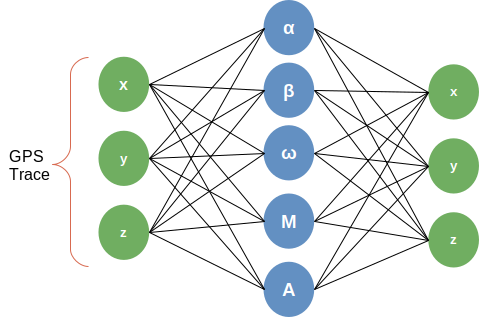
\includegraphics[width=0.6\textwidth]{neural_coding_gps.png}
        \end{figure}

        \begin{figure}[H]
            \centering
            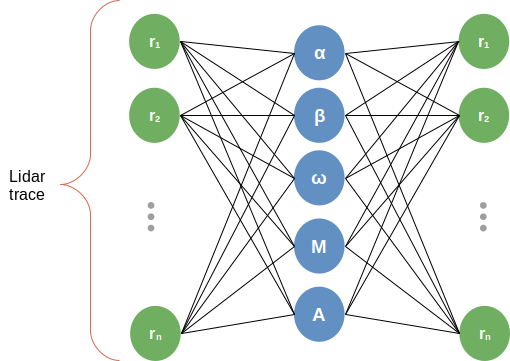
\includegraphics[width=0.6\textwidth]{neural_coding_lidar.png}
        \end{figure}
    \end{frame}

    \subsection{}
        \section{}
    \begin{frame}[allowframebreaks]{Frequency Modulated M\"obius (FMM)}
        
        
        \cite{rueda-2021-a-novel-wave-decomposition-for-oscillatory-signals} proposes a wave-decomposition method for oscillatory signals based on Frequency Modulated M\"obius (FMM) waves.
        
        \begin{equation}
            W(t)
            =
            M
            +
            A
            \cos
            \Biggl[
                \beta
                +
                2
                \arctan
                \Biggl(
                \omega
                \tan
                \Bigl(
                \frac{t-\alpha}{2}
                \Bigr)
                \Biggr)
                \Biggr]
        \end{equation}
        
        \begin{itemize}
            \item $W(t)$ is the value of the FMM wave at time $t$.
            \item $M$ is the baseline parameter. Bound: $M \in \mathbb{R}$. It controls the vertical shift of the FMM signal without changing the waveform shape, phase, or temporal deformation.
            
            \item $t$ is time. Bound: $t \in [0, 2\pi)$.
            
            \item $A$ is the amplitude parameter. Bound: $A \geq 0$. It controls the vertical scale of the waveform.
            
            \item $\alpha$ is the location parameter. Bound: $\alpha \in [0, 2\pi)$. It controls the horizontal position of the waveform on the time axis.
            
            \item $\beta$ is the phase parameter. Bound: $\beta \in [0, 2\pi)$. It controls the phase shift of the waveform. In other words, it determines, for example relative to $\alpha$, where the maximum point of the wave begins.
            
            \item $\omega$ is the shape parameter. Bound: $\omega \in (0, 1]$. It controls the sharpness, skewness, and temporal deformation of the waveform. It is defined in $(0, 1]$; in \cite{rueda-2021-a-novel-wave-decomposition-for-oscillatory-signals}, when it is close to 0 the waveform is more spike-like, whereas when it is near 1 it is more sinusoidal.
        \end{itemize}
        
        \alert{Why FMM to represent an action potential oscillatory wave?}\\
        This research uses variational autoencoders to encode a trace into the latent space of FMM-wave parameters. Why?
        \begin{itemize}
            \item Representing different sensory-data modalities in a unified form (i.e., both GPS and LiDAR are converted into FMM waves, each representing an action potential for a stimulus)
        \end{itemize}
        
    \end{frame}
        \section{}
    \begin{frame}[allowframebreaks]{Vector-Valued Sensor Composition}
        
        Composition and decomposition are based on orthogonal spaces for each sensor.
        \begin{block}{Why composing sensors}
            \begin{itemize}
                \item This is similar to what biological agents do (smell, touch, etc. are composed together)
                \item Computationally less expensive
            \end{itemize}
        \end{block}
        
        
        \begin{block}{Why?}
            \begin{itemize}
                \item The result is also an FMM representation (a unified form from sensation to anomaly representation)
                \item No need to train a Transformer for each sensor (first fuse, then train, then decompose)
            \end{itemize}
            
        \end{block}
        
        \small
        
        Each sensor reading is encoded into an FMM parameter vector:
        
        \begin{equation}
            \theta_t^i
            =
            (M_t^i,A_t^i,\alpha_t^i,\beta_t^i,\omega_t^i),
            \qquad
            i=1,\ldots,n
        \end{equation}
        
        Each parameter vector generates one sensor-specific FMM wave:
        
        \begin{equation}
            w_t^i(s)
            =
            \mathrm{FMM}(s;\theta_t^i),
            \qquad
            s \in [0,2\pi]
        \end{equation}
        
        The sensor-specific waves are composed on orthonormal sensor axes:
        
        \begin{equation}
            \mathbf{U}_t(s)
            =
            \sum_{i=1}^{n}
            w_t^i(s)\mathbf{e}_i,
            \qquad
            \mathbf{e}_i^{\top}\mathbf{e}_j
            =
            \delta_{ij}
        \end{equation}
        
        Therefore, the composed representation is a vector-valued wave:
        
        \begin{equation}
            \mathbf{U}_t(s)
            =
            \begin{bmatrix}
                w_t^1(s) \\
                w_t^2(s) \\
                \vdots \\
                w_t^n(s)
            \end{bmatrix}
        \end{equation}
        
        \[
            \text{Composition preserves sensor identity inside one shared temporal representation.}
        \]
    
    
    \end{frame}
        \section{}
    \begin{frame}[allowframebreaks]{Vector-Valued Sensor Composition example}


        \begin{figure}[H]
            \centering
            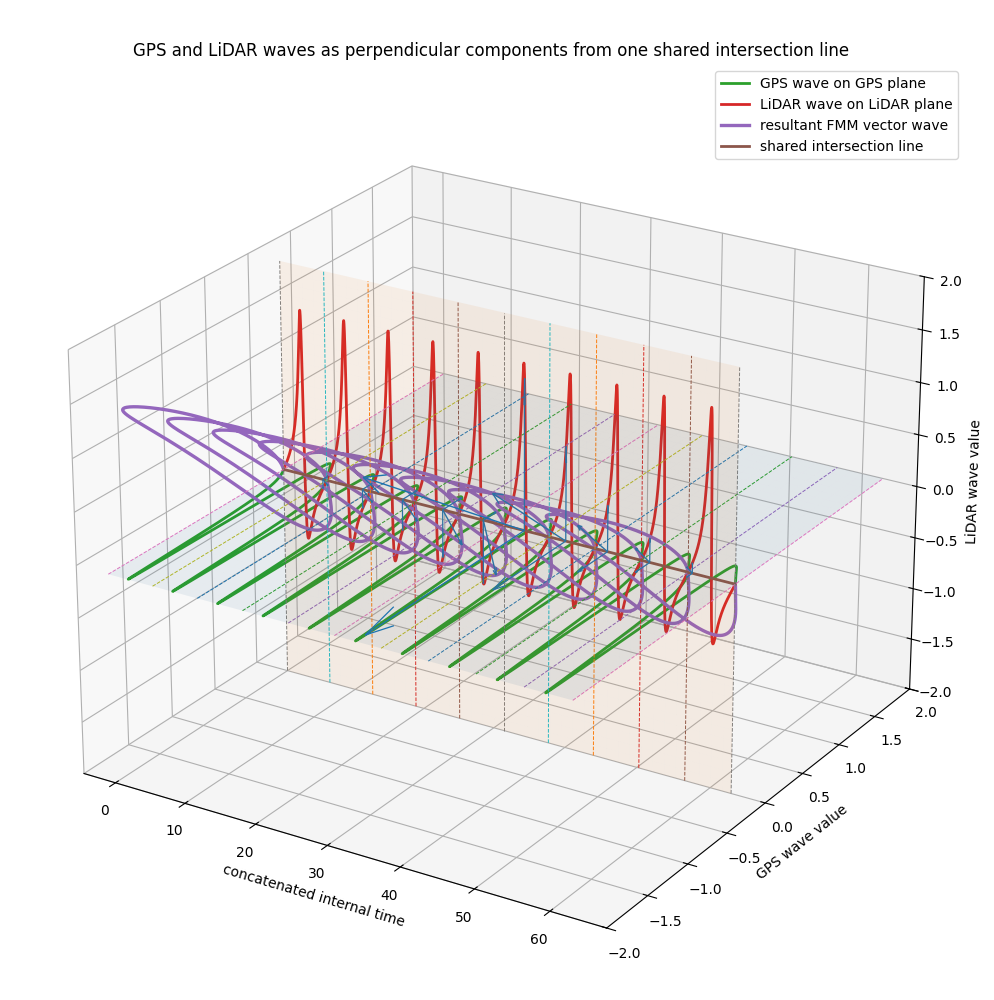
\includegraphics[width=0.8\textwidth]{frequency_modulated_mobius_composition_example.png}
        \end{figure}

    \end{frame}

        \section{}
    \begin{frame}[allowframebreaks]{Approximate Sensor Decomposition}
        
        
        \small
        
        After temporal prediction, the model produces a predicted vector-valued wave:
        
        \begin{equation}
            \hat{\mathbf{U}}_{t+1}(s)
            =
            \begin{bmatrix}
                \hat{w}_{t+1}^1(s) \\
                \hat{w}_{t+1}^2(s) \\
                \vdots \\
                \hat{w}_{t+1}^n(s)
            \end{bmatrix}
        \end{equation}
        
        Each sensor-specific wave is extracted by projection:
        
        \begin{equation}
            \hat{w}_{t+1}^i(s)
            =
            \hat{\mathbf{U}}_{t+1}(s)^{\top}
            \mathbf{e}_i,
            \qquad
            i=1,\ldots,n
        \end{equation}
        
        The corresponding FMM parameter vector is then estimated:
        
        \begin{equation}
            \hat{\theta}_{t+1}^i
            \approx
            \operatorname{Decompose}_i
            (
            \hat{w}_{t+1}^i
            )
        \end{equation}
        
        where:
        
        \begin{equation}
            \hat{\theta}_{t+1}^i
            =
            (
            \hat{M}_{t+1}^i,
            \hat{A}_{t+1}^i,
            \hat{\alpha}_{t+1}^i,
            \hat{\beta}_{t+1}^i,
            \hat{\omega}_{t+1}^i
            )
        \end{equation}
        
        Finally, the sensor decoder reconstructs the predicted sensor reading:
        
        \begin{equation}
            \hat{S}_{t+1}^i
            =
            \operatorname{Decoder}_i
            (
            \hat{\theta}_{t+1}^i
            )
        \end{equation}
        
        \[
            \text{Decomposition estimates the most likely sensor-specific contributors.}
        \]
    
    \end{frame}
        \begin{frame}[allowframebreaks]{Action potential simulation from sensory data}
    \cite{shimazaki-2025-neural-coding-foundational-concepts-statistical-formulations-and-recent-advances} Transformation of neural activity into perception and behavior by combining classical concepts with statistical encoding and decoding frameworks.
    \begin{figure}[H]
        \centering
        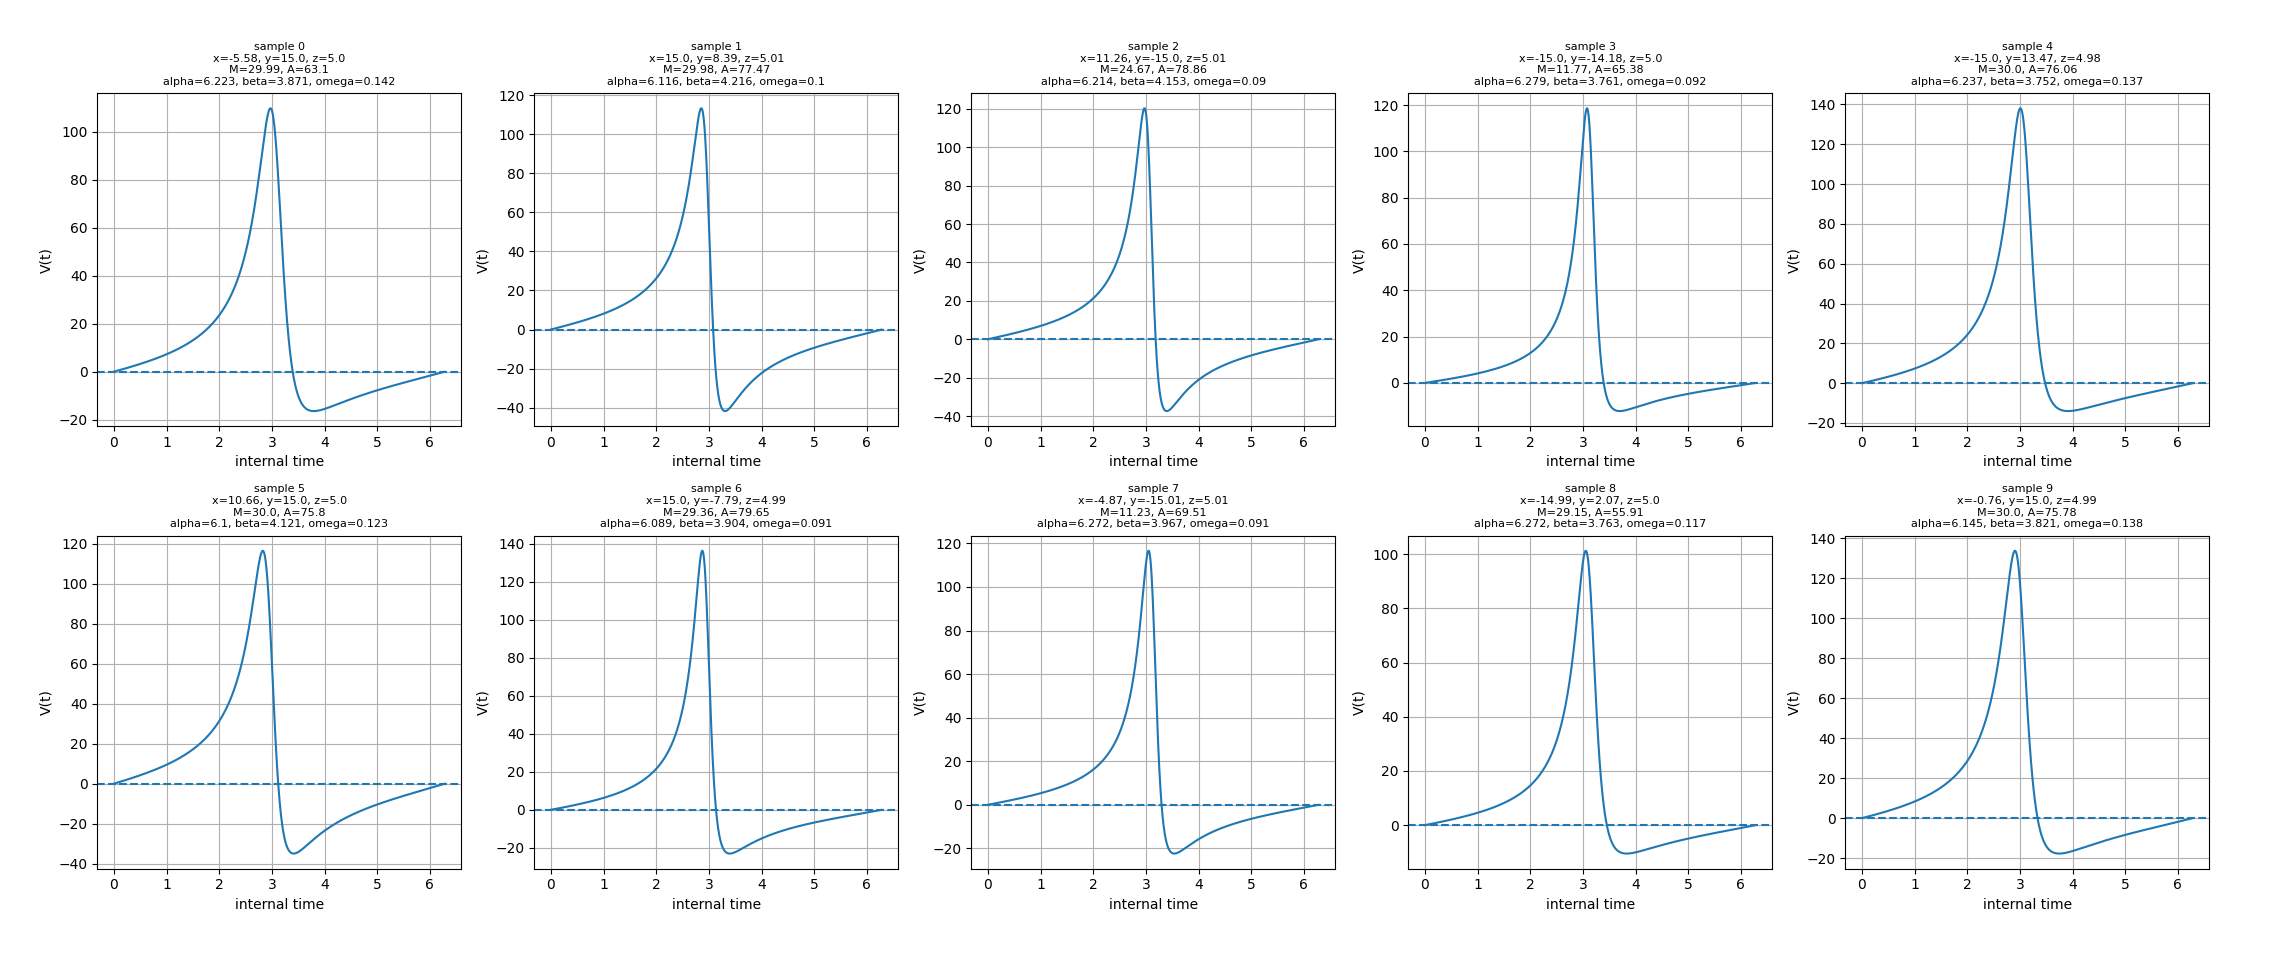
\includegraphics[width=0.6\textwidth]{gps_encoding.png}
    \end{figure}
\end{frame}

        \begin{frame}[allowframebreaks]{Action potential simulation from sensory data}
    \cite{shimazaki-2025-neural-coding-foundational-concepts-statistical-formulations-and-recent-advances} Transformation of neural activity into perception and behavior by combining classical concepts with statistical encoding and decoding frameworks.
    \begin{figure}[H]
        \centering
        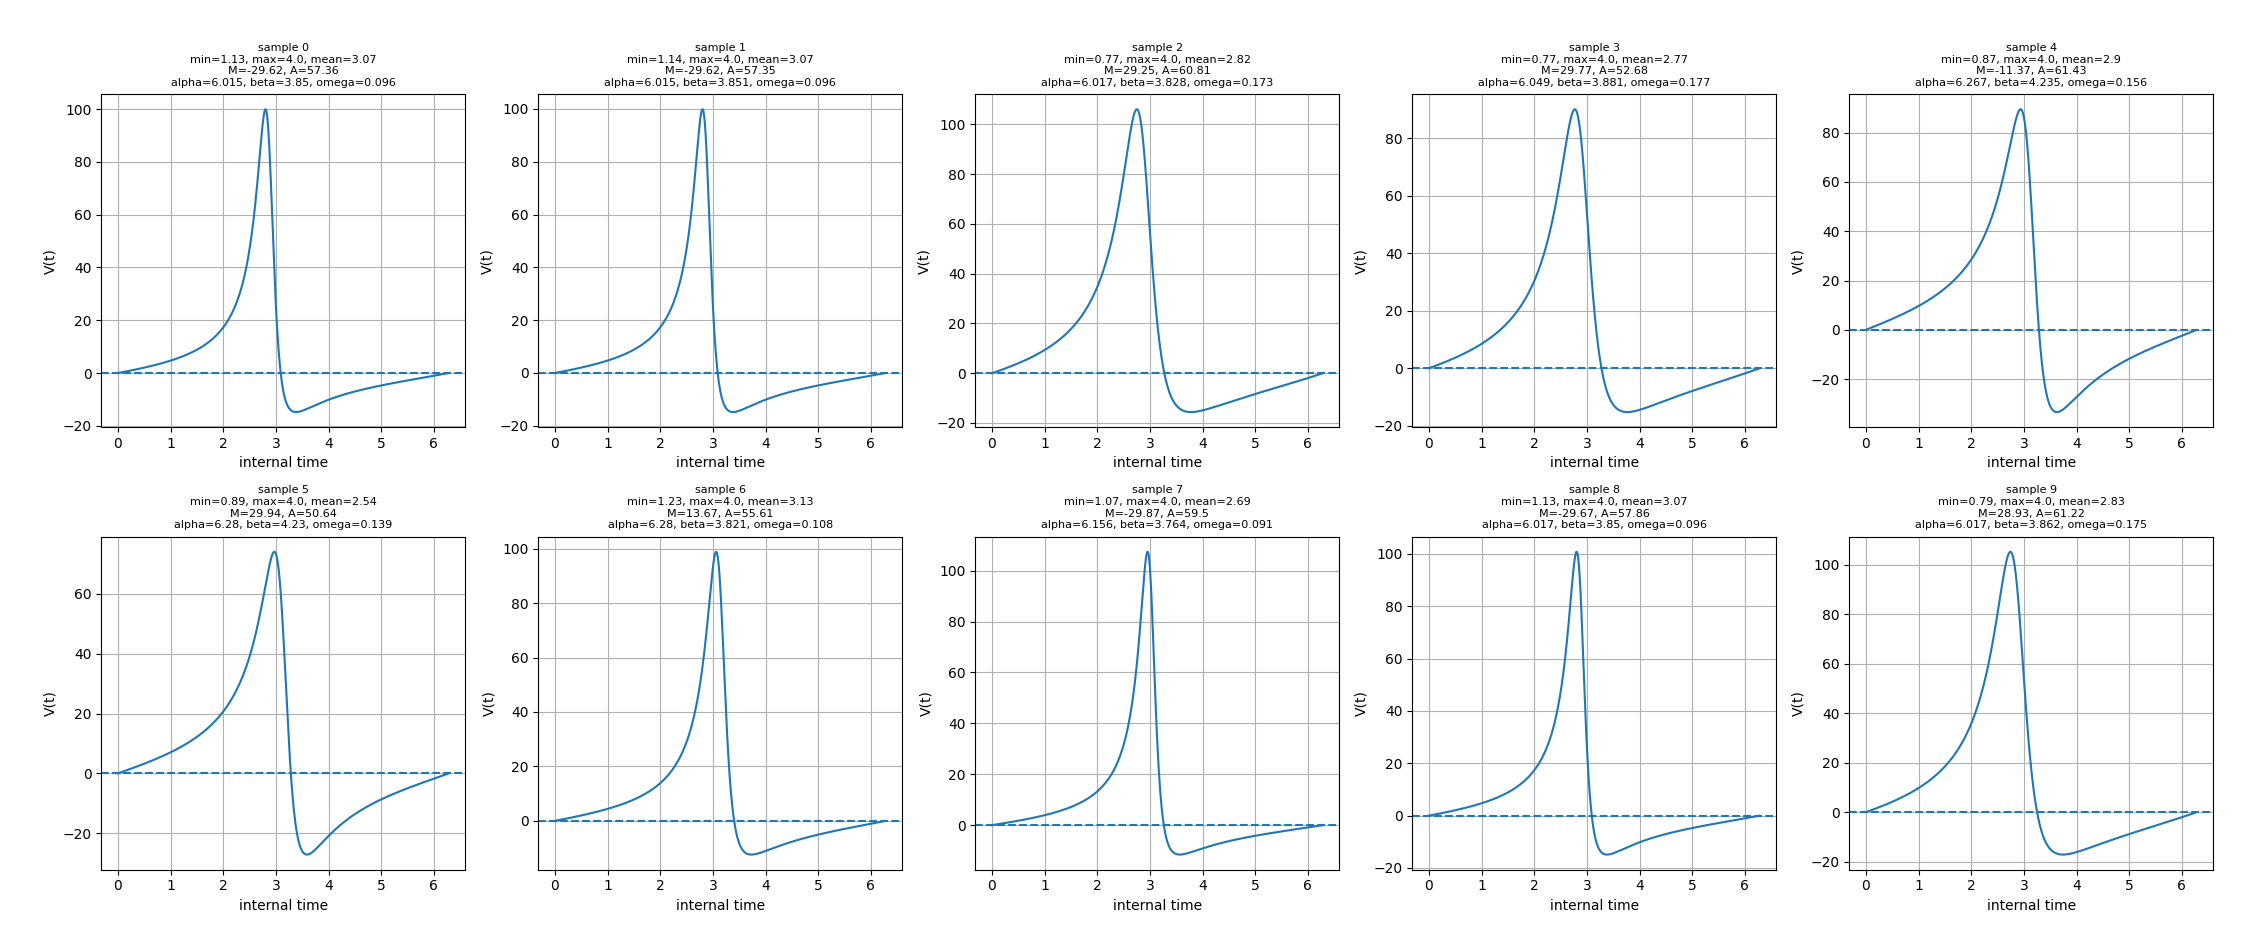
\includegraphics[width=0.6\textwidth]{lidar_encoding.png}
    \end{figure}
\end{frame}

